\chapter{Сұрыптау}

\index{сұрыптау}

\key{Сұрыптау} --
алгоритмдерді жобалаудағы іргелі әдіс-тәсілдердің бірі.
Ол көптеген тиімді алгоритмдерде ішбағдарлама ретінде қолданылады. Өйткені сұрыпталған енгізулермен есеп оңай шығарылады.

Мысалы, ''жиымда екі бірдей элемент бар ма?'' деген сұраққа
сұрыптау арқылы жауап берген ыңғайлы. Жиымда екі бірдей элемент болса, сұрыптаудан кейін олар бір-бірінің жанына орналасады.
Осылайша олар оңай анықталады.
Сонымен қатар ''ең жиі кездесетін элементті табу'' есебін де ұқсас жолмен шеше аламыз.

Сұрыптау алгоритмдері өте көп, және оларды өзге алгоритмдерді құруда үлгі ретінде алуға болады.
Тиімді жалпы сұрыптау алгоритмдері
$O(n \log n)$ уақытта жұмыс жасайды.
Сұрыптауды ішбағдарлама ретінде қолданатын алгоритмдердің уақытша күрделілігі де көбіне соған тең болып келеді.

\section{Сұрыптау теориясы}

Сұрыптаудағы негізгі есептердің бірі :
\begin{framed}
\noindent
$n$ элементтен тұратын жиым берілген,
оны өсу реті бойынша жүйеге келтіруіміз қажет.
\end{framed}
\noindent
Мысалы, мына жиым
\begin{center}
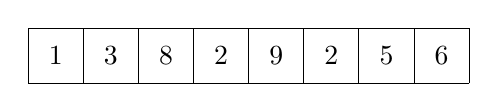
\begin{tikzpicture}[scale=0.7]
\draw (0,0) grid (8,1);
\node at (0.5,0.5) {$1$};
\node at (1.5,0.5) {$3$};
\node at (2.5,0.5) {$8$};
\node at (3.5,0.5) {$2$};
\node at (4.5,0.5) {$9$};
\node at (5.5,0.5) {$2$};
\node at (6.5,0.5) {$5$};
\node at (7.5,0.5) {$6$};
\end{tikzpicture}
\end{center}
сұрыптаудан кейін төмендегідей болып өзгереді:
\begin{center}
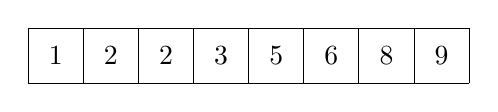
\begin{tikzpicture}[scale=0.7]
\draw (0,0) grid (8,1);
\node at (0.5,0.5) {$1$};
\node at (1.5,0.5) {$2$};
\node at (2.5,0.5) {$2$};
\node at (3.5,0.5) {$3$};
\node at (4.5,0.5) {$5$};
\node at (5.5,0.5) {$6$};
\node at (6.5,0.5) {$8$};
\node at (7.5,0.5) {$9$};
\end{tikzpicture}
\end{center}

\subsubsection{$O(n^2)$ алгоритмдері}

\index{көпіршікті сұрыптау}

Қарапайым сұрыптау алгоритмдері $O(n^2)$ 
уақытта жұмыс жасайды.
Олар ықшам болады және әдетте екі циклден тұрады.
$O(n^2)$ уақытта жұмыс істейтін сұрыптау алгоритмдерінің ішіндегі ең танымалы -- \key{көпіршікті сұрыптау}.
Ол $n$ кезеңнен тұрады.
Әр кезеңде алгоритм жиым ішімен өтіп шығады.
Екі қатар келетін элемент бұрыс тұрса,
оларды алмастырады.

Алгоритм төменде көрсетілген жолмен орындалады:
\begin{lstlisting}
for (int i = 0; i < n; i++) {
    for (int j = 0; j < n-1; j++) {
        if (array[j] > array[j+1]) {
            swap(array[j],array[j+1]);
        }
    }
}
\end{lstlisting}

1-кезеңнен кейін
ең үлкен элемент өз орнына келеді,
сәйкесінше $k$ кезеңнен соң $k$ үлкен сан 
нақты өз орнында болады.
Осылайша, $n$ кезеңде барлық жиымды сұрыптай аламыз.

Мысалы, жиымда

\begin{center}
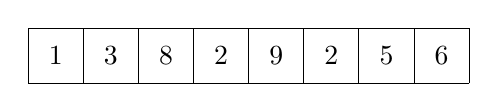
\begin{tikzpicture}[scale=0.7]
\draw (0,0) grid (8,1);

\node at (0.5,0.5) {$1$};
\node at (1.5,0.5) {$3$};
\node at (2.5,0.5) {$8$};
\node at (3.5,0.5) {$2$};
\node at (4.5,0.5) {$9$};
\node at (5.5,0.5) {$2$};
\node at (6.5,0.5) {$5$};
\node at (7.5,0.5) {$6$};
\end{tikzpicture}
\end{center}

\noindent
1-кезеңдегі алмасулар:

\begin{center}
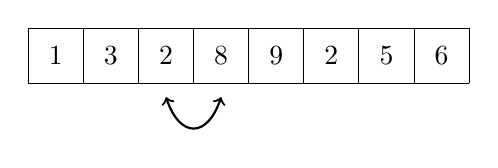
\begin{tikzpicture}[scale=0.7]
\draw (0,0) grid (8,1);
\node at (0.5,0.5) {$1$};
\node at (1.5,0.5) {$3$};
\node at (2.5,0.5) {$2$};
\node at (3.5,0.5) {$8$};
\node at (4.5,0.5) {$9$};
\node at (5.5,0.5) {$2$};
\node at (6.5,0.5) {$5$};
\node at (7.5,0.5) {$6$};

\draw[thick,<->] (3.5,-0.25) .. controls (3.25,-1.00) and (2.75,-1.00) .. (2.5,-0.25);
\end{tikzpicture}
\end{center}

\begin{center}
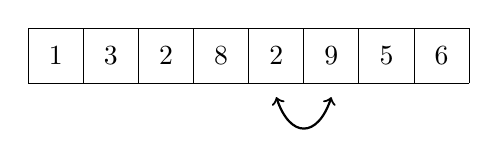
\begin{tikzpicture}[scale=0.7]
\draw (0,0) grid (8,1);
\node at (0.5,0.5) {$1$};
\node at (1.5,0.5) {$3$};
\node at (2.5,0.5) {$2$};
\node at (3.5,0.5) {$8$};
\node at (4.5,0.5) {$2$};
\node at (5.5,0.5) {$9$};
\node at (6.5,0.5) {$5$};
\node at (7.5,0.5) {$6$};

\draw[thick,<->] (5.5,-0.25) .. controls (5.25,-1.00) and (4.75,-1.00) .. (4.5,-0.25);
\end{tikzpicture}
\end{center}

\begin{center}
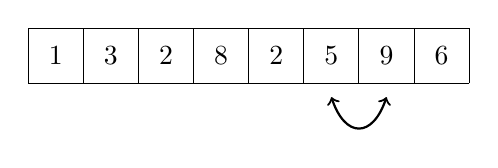
\begin{tikzpicture}[scale=0.7]
\draw (0,0) grid (8,1);
\node at (0.5,0.5) {$1$};
\node at (1.5,0.5) {$3$};
\node at (2.5,0.5) {$2$};
\node at (3.5,0.5) {$8$};
\node at (4.5,0.5) {$2$};
\node at (5.5,0.5) {$5$};
\node at (6.5,0.5) {$9$};
\node at (7.5,0.5) {$6$};

\draw[thick,<->] (6.5,-0.25) .. controls (6.25,-1.00) and (5.75,-1.00) .. (5.5,-0.25);
\end{tikzpicture}
\end{center}

\begin{center}
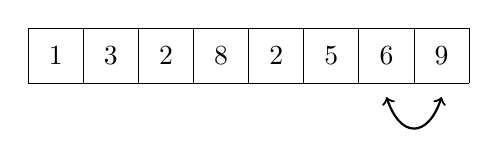
\begin{tikzpicture}[scale=0.7]
\draw (0,0) grid (8,1);
\node at (0.5,0.5) {$1$};
\node at (1.5,0.5) {$3$};
\node at (2.5,0.5) {$2$};
\node at (3.5,0.5) {$8$};
\node at (4.5,0.5) {$2$};
\node at (5.5,0.5) {$5$};
\node at (6.5,0.5) {$6$};
\node at (7.5,0.5) {$9$};

\draw[thick,<->] (7.5,-0.25) .. controls (7.25,-1.00) and (6.75,-1.00) .. (6.5,-0.25);
\end{tikzpicture}
\end{center}

\subsubsection{Инверсиялар}

\index{инверсиялар}

Көпіршікті сұрыптау \emph{қатар тұрған}
элементтерді алмастыру арқылы жүзеге асады.
Осылайша ол \emph{үнемі}
кем дегенде $O(n^2)$ уақытта жұмыс істейді.
Өйткені нашар жағдайда бізге
$O(n^2)$ алмастырулар жасауға тура келер еді.

Сұрыптау алгоритмдерін талдауда \key{инверсия}, яғни
элементтер жиымының 
$(\texttt{array}[a],\texttt{array}[b])$ жұбы үшін
$a<b$ және $\texttt{array}[a]>\texttt{array}[b]$ орындалып, элементтердің бұрыс ретпен орналасуы пайдалы болмақ.
Мысалы, келесі жиымда
\begin{center}
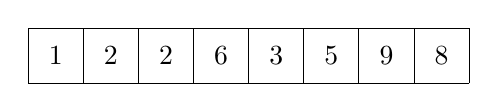
\begin{tikzpicture}[scale=0.7]
\draw (0,0) grid (8,1);
\node at (0.5,0.5) {$1$};
\node at (1.5,0.5) {$2$};
\node at (2.5,0.5) {$2$};
\node at (3.5,0.5) {$6$};
\node at (4.5,0.5) {$3$};
\node at (5.5,0.5) {$5$};
\node at (6.5,0.5) {$9$};
\node at (7.5,0.5) {$8$};
\end{tikzpicture}
\end{center}
үш инверсия бар: $(6,3)$, $(6,5)$ және $(9,8)$.
Инверсиялар саны
сұрыптау үшін қаншалықты жұмыс істеу қажеттілігін анықтайды.
Инверсияның болмауы жиымның сұрыпталғаны жайлы хабар береді.
Ал егер, жиым кері реттілікте болса,
инверсиялар санының болжамды ең үлкен мәні төмендегідей болмақ:
\[1+2+\cdots+(n-1)=\frac{n(n-1)}{2} = O(n^2)\]

Қате ретте орналасқан көршілес элементтер жұптарының алмасуы 
инверсиялар санын бірге азайтып отырады.
Осылайша, алгоритм жоғарыда келтірілген әрекет арқылы жүзеге асса, 
әр алмасу көп дегенде 1 инверсияны жойып отырады, 
сол себепті алгоритмнің уақытша күрделілігі қалай болғанда да $O(n^2)$.

\subsubsection{$O(n \log n)$ алгоритмдер}

\index{біріктіру бойынша сұрыптау}

Жиымды $O(n \log n)$ уақыт ішінде тезірек сұрыптауды
көршілес орналасқан элементтерді алмастырумен шектелмейтін
алгоритм арқылы да жүзеге асыру мүмкіндігі бар.
Осындай алгоритмдердің бірі рекурсияға негізделген 
\key{біріктіру бойынша сұрыптау деп аталады}\footnote{\cite{knu983}
мұндай сұрыптауды Дж. фон Нейман 1945 жылы ойлап тапты.}.

Ол \texttt{array}$[a \ldots b]$ ішжиымын төмендегідей сұрыптайды:

\begin{enumerate}
\item $a=b$ болған жағдайда, еш әрекет жасамаймыз, себебі ішжиым әлдеқашан сұрыпталған.
\item Центрде орналасқан элементтің позициясын анықтаймыз : $k=\lfloor (a+b)/2 \rfloor$.
\item Рекурсивті \texttt{array}$[a \ldots k]$ ішжиымын сұрыптаймыз.
\item \texttt{array}$[k+1 \ldots b]$ ішжиымын да дәл осылай сұрыптаймыз.
\item Сұрыпталған \texttt{array}$[a \ldots k]$ және
\texttt{array}$[k+1 \ldots b]$ ішжиымдарын \texttt{array}$[a \ldots b]$
\emph{біріктіреміз}.
\end{enumerate}

Бағдарламалауда бұл алгоритм тиімді саналады. Себебі 
ол әр қадам сайын ішжиым өлшемін екі есеге азайтып отырады.
Рекурсия $O(\log n)$ деңгейден тұрады
және әр деңгейді өңдеуге $O(n)$ уақыт кетеді.
Ал \texttt{array}$[a \ldots k]$ мен \texttt{array}$[k+1 \ldots b]$
ішжиымдарын біріктіру олар әлдеқашан сұрыпталғандықтан сызықты уақытты алады.

Мысалы, келесі жиымды сұрыптау жолын қарастырайық:
\begin{center}
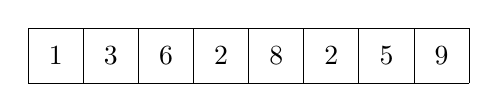
\begin{tikzpicture}[scale=0.7]
\draw (0,0) grid (8,1);
\node at (0.5,0.5) {$1$};
\node at (1.5,0.5) {$3$};
\node at (2.5,0.5) {$6$};
\node at (3.5,0.5) {$2$};
\node at (4.5,0.5) {$8$};
\node at (5.5,0.5) {$2$};
\node at (6.5,0.5) {$5$};
\node at (7.5,0.5) {$9$};
\end{tikzpicture}
\end{center}

Жиымды екіге бөлейік:
\begin{center}
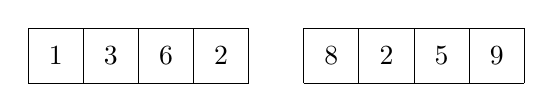
\begin{tikzpicture}[scale=0.7]
\draw (0,0) grid (4,1);
\draw (5,0) grid (9,1);

\node at (0.5,0.5) {$1$};
\node at (1.5,0.5) {$3$};
\node at (2.5,0.5) {$6$};
\node at (3.5,0.5) {$2$};

\node at (5.5,0.5) {$8$};
\node at (6.5,0.5) {$2$};
\node at (7.5,0.5) {$5$};
\node at (8.5,0.5) {$9$};
\end{tikzpicture}
\end{center}

Кейін ішжиымдар рекурсивті түрде сұрыпталады:
\begin{center}
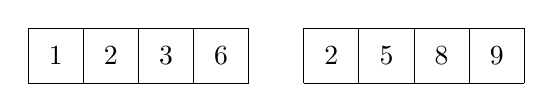
\begin{tikzpicture}[scale=0.7]
\draw (0,0) grid (4,1);
\draw (5,0) grid (9,1);

\node at (0.5,0.5) {$1$};
\node at (1.5,0.5) {$2$};
\node at (2.5,0.5) {$3$};
\node at (3.5,0.5) {$6$};

\node at (5.5,0.5) {$2$};
\node at (6.5,0.5) {$5$};
\node at (7.5,0.5) {$8$};
\node at (8.5,0.5) {$9$};
\end{tikzpicture}
\end{center}

Соңында алгоритм барлық ішжиымдардан 
сұрыпталған жиым құрайды:
\begin{center}
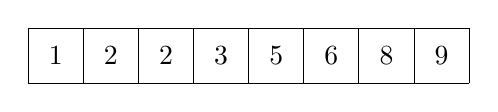
\begin{tikzpicture}[scale=0.7]
\draw (0,0) grid (8,1);
\node at (0.5,0.5) {$1$};
\node at (1.5,0.5) {$2$};
\node at (2.5,0.5) {$2$};
\node at (3.5,0.5) {$3$};
\node at (4.5,0.5) {$5$};
\node at (5.5,0.5) {$6$};
\node at (6.5,0.5) {$8$};
\node at (7.5,0.5) {$9$};
\end{tikzpicture}
\end{center}

\subsubsection{Сұрыптаудың төменгі шегі}

''$O(n \log n)$ уақытынан жылдамырақ сұрыптау мүмкін бе?'' -- деген заңды сұрақ туындайды. 
Бұл сұраққа: ''Егер алмастыру алгоритмдерімен шектелсек, мүмкін \emph{емес}'' -- деп жауап беруге болады. 

Уақытша күрделілігінің төменгі шегін дәлелдеу үшін
сұрыптауды әр салыстыру сайын жиым туралы молырақ
ақпарат беретін үдеріс деп қарастырайық.
Бұл үдерістен төмендегідей дарақ шығады:

\begin{center}
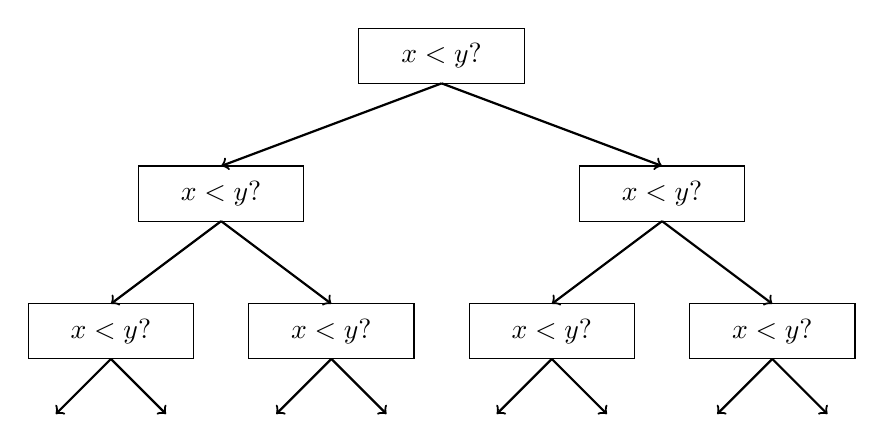
\begin{tikzpicture}[scale=0.7]
\draw (0,0) rectangle (3,1);
\node at (1.5,0.5) {$x < y?$};

\draw[thick,->] (1.5,0) -- (-2.5,-1.5);
\draw[thick,->] (1.5,0) -- (5.5,-1.5);

\draw (-4,-2.5) rectangle (-1,-1.5);
\draw (4,-2.5) rectangle (7,-1.5);
\node at (-2.5,-2) {$x < y?$};
\node at (5.5,-2) {$x < y?$};

\draw[thick,->] (-2.5,-2.5) -- (-4.5,-4);
\draw[thick,->] (-2.5,-2.5) -- (-0.5,-4);
\draw[thick,->] (5.5,-2.5) -- (3.5,-4);
\draw[thick,->] (5.5,-2.5) -- (7.5,-4);

\draw (-6,-5) rectangle (-3,-4);
\draw (-2,-5) rectangle (1,-4);
\draw (2,-5) rectangle (5,-4);
\draw (6,-5) rectangle (9,-4);
\node at (-4.5,-4.5) {$x < y?$};
\node at (-0.5,-4.5) {$x < y?$};
\node at (3.5,-4.5) {$x < y?$};
\node at (7.5,-4.5) {$x < y?$};

\draw[thick,->] (-4.5,-5) -- (-5.5,-6);
\draw[thick,->] (-4.5,-5) -- (-3.5,-6);
\draw[thick,->] (-0.5,-5) -- (0.5,-6);
\draw[thick,->] (-0.5,-5) -- (-1.5,-6);
\draw[thick,->] (3.5,-5) -- (2.5,-6);
\draw[thick,->] (3.5,-5) -- (4.5,-6);
\draw[thick,->] (7.5,-5) -- (6.5,-6);
\draw[thick,->] (7.5,-5) -- (8.5,-6);
\end{tikzpicture}
\end{center}

Бұл жердегі ''$x<y?$'' қандай да бір
$x$ пен $y$ элементтерінің салыстырылуын білдіреді.
Егер $x<y$ болса, үдеріс солға жалғасады.
Ал кері жағдайда оңға қарай ауысады.
Нәтижелер -- жиымды сұрыптаудың $n!$ болжамды жолдары.
Сол себепті, дарақтың биіктігі кем дегенде
\[ \log_2(n!) = \log_2(1)+\log_2(2)+\cdots+\log_2(n).\]
Қосындының төменгі шегін соңғы $n/2$ элементті таңдап,
әрқайсының мәнін $\log_2(n/2)$-ге өзгерту арқылы анықтай аламыз.
Беретін бағасы
\[ \log_2(n!) \ge (n/2) \cdot \log_2(n/2),\]
сондықтан дарақтың биіктігі мен сұрыптау
алгоритмі ең нашар жағдайда жасайтын 
минималды жүріс саны $n \log n$ - ге тең.

\subsubsection{Санамалы сұрыптау}

\index{санамалы сұрыптау}
$n \log n$ элементтерді салыстырмай,
өзге ақпараттарды қолдана отырып сұрыптайтын алгоритмдер
үшін төменгі шек бола алмайды.
Осындай алгоритмдердің бірі -- $O(n)$ уақытта жұмыс жасайтын
санамалы сұрыптау, ол жиымдағы элементтер $0 \ldots c$ 
аралығанда деген болжамға негізделген және $c=O(n)$.

Біз индекстері бастапқы жиымның элементтерімен сәйкес келетін көмекші жиымды қолданатын боламыз. Алгоритм бастапқы  жиымды айналып шығып, онда әр элементтің қанша рет кездесетінін есептейді.

Мысалы, мына жиымнан
\begin{center}
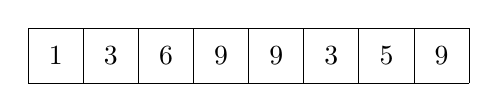
\begin{tikzpicture}[scale=0.7]
\draw (0,0) grid (8,1);
\node at (0.5,0.5) {$1$};
\node at (1.5,0.5) {$3$};
\node at (2.5,0.5) {$6$};
\node at (3.5,0.5) {$9$};
\node at (4.5,0.5) {$9$};
\node at (5.5,0.5) {$3$};
\node at (6.5,0.5) {$5$};
\node at (7.5,0.5) {$9$};
\end{tikzpicture}
\end{center}
келесі есептік жиым туындайды:
\begin{center}
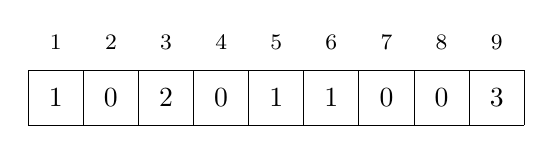
\begin{tikzpicture}[scale=0.7]
\draw (0,0) grid (9,1);
\node at (0.5,0.5) {$1$};
\node at (1.5,0.5) {$0$};
\node at (2.5,0.5) {$2$};
\node at (3.5,0.5) {$0$};
\node at (4.5,0.5) {$1$};
\node at (5.5,0.5) {$1$};
\node at (6.5,0.5) {$0$};
\node at (7.5,0.5) {$0$};
\node at (8.5,0.5) {$3$};

\footnotesize

\node at (0.5,1.5) {$1$};
\node at (1.5,1.5) {$2$};
\node at (2.5,1.5) {$3$};
\node at (3.5,1.5) {$4$};
\node at (4.5,1.5) {$5$};
\node at (5.5,1.5) {$6$};
\node at (6.5,1.5) {$7$};
\node at (7.5,1.5) {$8$};
\node at (8.5,1.5) {$9$};
\end{tikzpicture}
\end{center}

Есептік жиымның 3-индексінде
2 саны сақталған, себебі
3 элементі негізгі жиымда 2 рет кездеседі.

Аталған жиым $O(n)$ уақытта құрылады. Ал сұрыпталған
жиым құрау $O(n)$ уақыт алады. Себебі әр элементтің 
қанша рет кездескенін есептік жиымнан біле аламыз.
Сондықтан санамалы сұрыптаудың уақытша күрделілігі $O(n)$-ге тең.

Тұрақты $c$ жеткілікті деңгейде кіші болған
жағдайда есептік жиым құру мүмкіндігі артады.
Сондықтан санамалы сұрыптау өте тиімді алгоритм болмақ.

\section{C++ -тегі сұрыптау}

\index{sort@\texttt{sort}}

Контестте қолдан құрастырылған сұрыптау алгоритмін пайдалану сирек жағдайларда ғана жақсы идея деп саналады. Өйткені бағдарламалау тілдерінде
кірістірілген жақсы тәсілдер баршылық.
Мысалы, C++ стандартты дерекханасында \texttt{sort}
функциясы бар, оның көмегімен жиымдар және басқа да деректер
құрылымдарын оңай сұрыптай аламыз.

Дерекхананың сұрыптау функциясын пайдаланудың
көптеген артықшылықтары бар.
Біріншіден, ол уақытты үнемдейді. Себебі функция кодын жазуға уақыт кетпейді.
Екіншіден, оның жүзеге асыру тәсілі тиімді әрі дұрыс. Өйткені қолдан құрастырылған алгоритмнің жақсырақ болуы екіталай.

Бұл бөлікте C++ \texttt{sort} функциясын 
қолдану барысын қарастырамыз.
Келесі код векторды өсу ретімен сұрыптайды:
\begin{lstlisting}
vector<int> v = {4,2,5,3,5,8,3};
sort(v.begin(),v.end());
\end{lstlisting}
Сұрыптаудан кейінгі вектор
$[2,3,3,4,5,5,8]$.
Әдепкі қалпы бойынша жұмыс істесе, өсу реті бойынша жүзеге асады,
бірақ кері ретпен сұрыптауды төмендегіше орындай аламыз:
\begin{lstlisting}
sort(v.rbegin(),v.rend());
\end{lstlisting}
Кәдімгі жиым осылай реттеледі:
\begin{lstlisting}
int n = 7; // array size
int a[] = {4,2,5,3,5,8,3};
sort(a,a+n);
\end{lstlisting}

Ал \texttt{s} жолын сұрыптау төмендегідей орындалады:
\begin{lstlisting}
string s = "monkey";
sort(s.begin(), s.end());
\end{lstlisting}
Жолды сұрыптау дегеніміз оның құрамындағы 
элементтердің реттелуін білдіреді.
Мысалы, ''monkey'' жолы ''ekmnoy'' болып өзгереді.

\subsubsection{Салыстыру операторлары}

\index{салыстыру операторлары}

\texttt{sort} функциясы элементтерді сұрыптау кезінде
дерек типіне байланысты салыстыру  операторын талап етеді.
Оператор екі элементтің орындарын анықтауда қажет.

Көптеген C++ дерек типтерінің кірістірілген
салыстыру операторлары болады, сондықтан элементтер 
автоматты түрде сұрыптала алады.
Мысалы, сандар мәндеріне байланысты, ал жолдар әліпбидегі
реттілігіне байланысты сұрыпталады.

\index{жұп@\texttt{жұп}}

(\texttt{pair}) жұптары бірінші элементтері 
(\texttt{first}) бойынша сұрыпталады.
Екі жұптың бірінші элементтері бірдей болса, екінші элементтері 
(\texttt{second}) бойынша реттеледі:
\begin{lstlisting}
vector<pair<int,int>> v;
v.push_back({1,5});
v.push_back({2,3});
v.push_back({1,2});
sort(v.begin(), v.end());
\end{lstlisting}
Осыдан кейінгі жұптардың реттілігі:
$(1,2)$, $(1,5)$ және $(2,3)$.

\index{кортеж@\texttt{кортеж}}

(\texttt{tuple}) кортеждері ұқсас жолмен 
алғашқы ретте бірінші элемент бойынша, кейін
екінші элемент бойынша, т.с.с. сұрыпталады 
\footnote{Кей ескі компиляторларда кортеж  
құрау үшін өрнек жақшалар орнына \texttt{make\_tuple}
функциясы қолданылуы қажет екенін ескерген жөн
(мысалы, \texttt{\{2,1,4\}} орнына 
\texttt{make\_tuple(2,1,4)}).}:
\begin{lstlisting}
vector<tuple<int,int,int>> v;
v.push_back({2,1,4});
v.push_back({1,5,3});
v.push_back({2,1,3});
sort(v.begin(), v.end());
\end{lstlisting}
Кейін кортеждер реттілігі осылай өзгереді:
$(1,5,3)$, $(2,1,3)$ және $(2,1,4)$.


\subsubsection{Пайдаланушы құрылымдары (struct)}

Пайдаланушы құрылымдарында (struct) автоматты түрдегі 
салыстыру операторлары болмайды.
Оператор құрылым (struct) ішінде параметрі сол типтегі 
элемент болатын \texttt{operator<} 
функциясы ретінде анықталуы қажет.
Ол элемент параметрден кішірек болса, \texttt{true} арқылы, 
кері жағдайда \texttt{false} арқылы қайтару керек.

Мысалы, кезекті struct \texttt{P}
x және y координатты нүктелерін қамтиды.
Салыстыру операторы бірінші x координаты,
ал кейін y координаты бойынша сұрыптайды.

\begin{lstlisting}
struct P {
    int x, y;
    bool operator<(const P &p) {
        if (x != p.x) return x < p.x;
        else return y < p.y;
    }
};
\end{lstlisting}

\subsubsection{Салыстыру функциялары}

\index{салыстыру функциясы}

\key{Салыстырудың сыртқы функциясын} да солай анықтап, 
оның \texttt{sort} функциясын кері шақыру функциясы ретінде беруге болады.
Мысалы, келесі \texttt{comp} салыстыру функциясы 
жолды бірінші кезекте ұзындығы бойынша, ал егер екі
бірдей ұзындықтағы жол кездессе, әліпбидегі реттіліктері
бойынша сұрыптайды:

\begin{lstlisting}
bool comp(string a, string b) {
    if (a.size() != b.size()) return a.size() < b.size();
    return a < b;
}
\end{lstlisting}
Жолдардан тұратын вектор осылай сұрыпталады:
\begin{lstlisting}
sort(v.begin(), v.end(), comp);
\end{lstlisting}

\section{Бинарлық ізденіс}

\index{бинарлық ізденіс}

Жиымдағы элементті іздеудің негізгі жолы -- \texttt{for} 
қайталымы арқылы жиыммен өтіп шығу.
Мысалы, келесі код жиымнан
$x$ элементін іздейді:

\begin{lstlisting}
for (int i = 0; i < n; i++) {
    if (array[i] == x) {
        // x found at index i
    }
}
\end{lstlisting}

Тәсілдің уақытша күрделілігі $O(n)$, себебі ең нашар жағдайда
жиымның барлық элементін қарап шығуға мәжбүрміз.
Элементтер кез келген ретте орналасса, тәсіл біз үшін тиімді саналады.
Себебі $x$-ті қайдан іздестіру керектігі туралы қосымша ақпарат ала алмаймыз.

Егер жиым \emph{сұрыпталған} болса, жағдай басқаша қабылданады.
Бұл жағдайда іздестіруді реттілік көмегімен 
тез жүзеге асыра аламыз.
\key{Бинарлық ізденіс} алгоритмі сұрыпталған жиымнан
элементті $O(\log n)$ уақытта тиімді таба алады.

\subsubsection{Бірінші тәсіл}

Алгоритмді жүзеге асырудың қарапайым жолы -- сөздіктен 
сөз іздеуге ұқсас. Ізденісті алдымен жиымның барлық 
элементтерін қамтитын аралықтан бастаймыз.
Кейін бірнеше қадам ішінде аралықтың өлшемін 
екі есеге азайтып отырамыз.

Әр қадам сайын ізденіс қарастырылып жатқан
аралықтың орталық элементін тексереді.
Егер орталық элемент іздестірілген элемент болса,
ізденісті тоқтатамыз.
Басқа жағдайда, ізденіс орталық элементтің мәніне байланысты
оң жаққа немесе сол жаққа жалғасады.

Идеяның орындалу жолы:
\begin{lstlisting}
int a = 0, b = n-1;
while (a <= b) {
    int k = (a+b)/2;
    if (array[k] == x) {
        // x found at index k
    }
    if (array[k] > x) b = k-1;
    else a = k+1;
}
\end{lstlisting}

Бұл жердегі қарастырылып жатқан аралық -- $a \ldots b$,
бастапқы қалпы -- $0 \ldots n-1$ аралығы.
Алгоритм әр қадамда ізденіс аралығын екі есеге кішірейтеді. Демек оның уақытша күрделілігі $O(\log n)$ болады. 

\subsubsection{Екінші тәсіл}

Біз бинарлық ізденісті басқа тәсілмен де жүзеге асыра аламыз. Ол үшін жиым элементтерінен тиімді өтіп шығу керек. Мұндағы идея секіруге және нысанға
жақындаған сайын жылдамдықты азайтуға негізделеді.

Ізденіс солдан оңға қарай жүреді, бастапқы секіріс --
$n/2$. Әр қадамда секіру ұзындығы екі есеге қысқарады:
алғашында $n/4$, кейін $n/8$, $n/16$, т.с.с., ақырғы 
ұзындық бір болғанға дейін жалғасады.
Секірістердің соңында біз нысандағы элементті табамыз
немесе оның жиымда жоқ екеніне көз жеткіземіз.
\newpage

Төменде осы идея бойынша жазылған код берілген:
\begin{lstlisting}
int k = 0;
for (int b = n/2; b >= 1; b /= 2) {
    while (k+b < n && array[k+b] <= x) k += b;
}
if (array[k] == x) {
    // x found at index k
}
\end{lstlisting}

Ізденіс барысында $b$ айнымалысы
секіріс ұзындығына жауап береді.
алгоритмнің уақытша күрделілігі -- $O(\log n)$.
Себебі кодтағы \texttt{while} айнымалысы
әр секіру ұзындығы үшін ең көп дегенде екі
рет қолданылады.

\subsubsection{C++ функциялары}

С++ стандартты дерекханасы бинарлық ізденіске 
негізделген және логарифмдік уақытта жұмыс істейтін
келесі функцияларды қамтиды:

\begin{itemize}
\item \texttt{lower\_bound} жиымдағы мәні кемінде $x$ болатын
бірінші элементке нұсқайды.
\item \texttt{upper\_bound} жиымдағы мәні $x$-тен үлкен ең
бірінші элементке нұсқайды.
\item \texttt{equal\_range} жоғарыдағы екеуін де қайтарады.
\end{itemize}

Функция жиым сұрыпталған деп қабылдайды.
Егер қажет элемент табылмаса, нұсқағыш жиымның соңғы
элементінен кейінгі элементке нұсқайды. 
Мысалы, төмендегі код жиымда $x$ элементі бар-жоғын анықтайды:

\begin{lstlisting}
auto k = lower_bound(array,array+n,x)-array;
if (k < n && array[k] == x) {
    // x found at index k
}
\end{lstlisting}

Ал келесі код $x$ жиымда қанша рет кездесетінін есептейді:

\begin{lstlisting}
auto a = lower_bound(array, array+n, x);
auto b = upper_bound(array, array+n, x);
cout << b-a << "\n";
\end{lstlisting}

\texttt{equal\_range} көмегімен кодты ықшамдай аламыз:

\begin{lstlisting}
auto r = equal_range(array, array+n, x);
cout << r.second-r.first << "\n";
\end{lstlisting}

\subsubsection{Ең кіші шешімді табу}

Бинарлық ізденістің маңызды қолданыс аясы --
функцияның мәні өзгеретін позицияны анықтау.
Есепке шешім бола алатын ең төмен $k$ мәнін
тапқымыз келеді делік.
Бізде $x$ жауап бола алса, \texttt{true}, басқа жағдайда
\texttt{false} қайтаратын $\texttt{ok}(x)$ функциясы бар.
Оған қоса, $\texttt{ok}(x)$ $x<k$ болғанда, \texttt{false}
және $x \ge k$ болғанда, \texttt{true} қайтаратынын білеміз.
Жағдаят көрінісі:

\begin{center}
\begin{tabular}{r|rrrrrrrr}
$x$ & 0 & 1 & $\cdots$ & $k-1$ & $k$ & $k+1$ & $\cdots$ \\
\hline
$\texttt{ok}(x)$ & \texttt{false} & \texttt{false}
& $\cdots$ & \texttt{false} & \texttt{true} & \texttt{true} & $\cdots$ \\
\end{tabular}
\end{center}

\noindent
$k$ мәнін бинарлық ізденіс арқылы анықтай аламыз:

\begin{lstlisting}
int x = -1;
for (int b = z; b >= 1; b /= 2) {
    while (!ok(x+b)) x += b;
}
int k = x+1;
\end{lstlisting}

$\texttt{ok}(x)$ \texttt{false} болатындай 
$x$-тің ең үлкен мәнін іздейміз. Осылайша, $k=x+1$
$\texttt{ok}(k)$ \texttt{true} болатындай
ең кіші мәнге тең.
Бастапқы секіріс ұзындығы $z$ жеткілікті
деңгейде үлкен болуы қажет,
мысалы біз алдын ала білетін қандай да бір
$\texttt{ok}(z)$ \texttt{true} болатын мән.

Алгоритм \texttt{ok} функциясын 
$O(\log z)$ рет шақырады, сол себепті
уақытша күрделілігі \texttt{ok} функциясына тәуелді.
Мысалы, функция $O(n)$ уақытта жұмыс жасаса,
жалпы уақытша күрделілігі -- $O(n \log z)$.

\subsubsection{Ең үлкен мәнді табу}

Сонымен қатар бинарлық ізденіс
мәні алдымен өсіп, кейін белгілі бір сәтте
күрт азаятын функция үшін де пайдаланылады.
Біздің тапсырмамыз төмендегідей $k$ мәнін табу

\begin{itemize}
\item
 $x<k$ үшін $f(x)<f(x+1)$, ал
\item
$x \ge k$ үшін $f(x)>f(x+1)$.
\end{itemize}

Идеясы -- $f(x)<f(x+1)$ болатын ең үлкен
$x$-ті бинарлық ізденіс арқылы табу. 
Бұл $k=x+1$ екенін білдіреді. Себебі
$f(x+1)>f(x+2)$. Төмендегі код 
ізденісті жүзеге асырады:

\begin{lstlisting}
int x = -1;
for (int b = z; b >= 1; b /= 2) {
    while (f(x+b) < f(x+b+1)) x += b;
}
int k = x+1;
\end{lstlisting}

Қарапайым бинарлық ізденістен айырмашылығы --
функцияның қатар келетін мәндері бірдей 
болуына рұқсат етілмейді. Бұл жағдайда ізденісті қалай
жалғастыру керектігін білу мүмкін емес. 
